\documentclass[border=3pt]{standalone}
% Preâmbulo compartilhado pelos diagramas TikZ da aula 10 de IHC (Planejamento da Avaliação)
\usepackage[T1]{fontenc}
\usepackage[utf8]{inputenc}
\usepackage{lmodern}
\usepackage{amsmath}
\usepackage{xcolor}
\usepackage{tikz}
\usetikzlibrary{arrows.meta,angles,quotes,decorations.pathmorphing,decorations.pathreplacing,calc,
                positioning,shapes.geometric,shapes.misc,backgrounds,fit,
                math}

% Paleta (mesma dos SVGs originais)
% Paleta da disciplina de IHC: acento roxo (#755099), da capa do livro.
% (o nome "dblue" é mantido para não alterar todos os diagramas)
\definecolor{dblue}{HTML}{755099}
\definecolor{dorange}{HTML}{B3541E}
\definecolor{dgreen}{HTML}{4A7C59}
\definecolor{dred}{HTML}{9C4B4B}
\definecolor{dcream}{HTML}{F4F1EA}
\definecolor{dshade}{HTML}{DDD7C9}

% Função gaussiana (não normalizada por padrão de escala visual)
\pgfmathdeclarefunction{gauss}{3}{%
  \pgfmathparse{1/(#3*sqrt(2*pi))*exp(-((#1-#2)^2)/(2*#3^2))}%
}

% Estilos comuns (prefixo d... para não colidir com chaves internas do pgf)
\tikzset{
  >={Stealth[length=2mm]},
  dguide/.style={gray!55, dashed, line width=0.4pt},
  daxis/.style={gray!60, line width=0.7pt, ->},
  dbody/.style={fill=black!3, draw=black!80, line width=1pt},
  dacc/.style={draw=dblue, line width=1pt},
  dlbl/.style={black!55, font=\small},
  dsub/.style={black!45, font=\footnotesize},
  dstate/.style={circle, draw=black!80, fill=dcream, line width=1pt,
                 minimum size=17mm, font=\large, inner sep=1pt},
  dobs/.style={circle, draw=black!80, fill=dshade, line width=1pt,
               minimum size=14mm, font=\large, inner sep=1pt},
  dbox/.style={rounded corners=2pt, draw=black!80, fill=dcream, line width=1pt,
               align=center, inner sep=6pt},
  dop/.style={circle, draw=black!80, fill=white, line width=1pt,
              minimum size=6mm, inner sep=0pt, font=\small},
  dtrans/.style={->, dblue, line width=1pt},
  dmeas/.style={->, dorange, line width=1pt},
  dcurve/.style={line width=1pt, dblue},
  dcurveb/.style={line width=1.4pt, dorange},
}

\begin{document}
\hyphenpenalty=10000 \exhyphenpenalty=10000 \tolerance=9999 \emergencystretch=3em
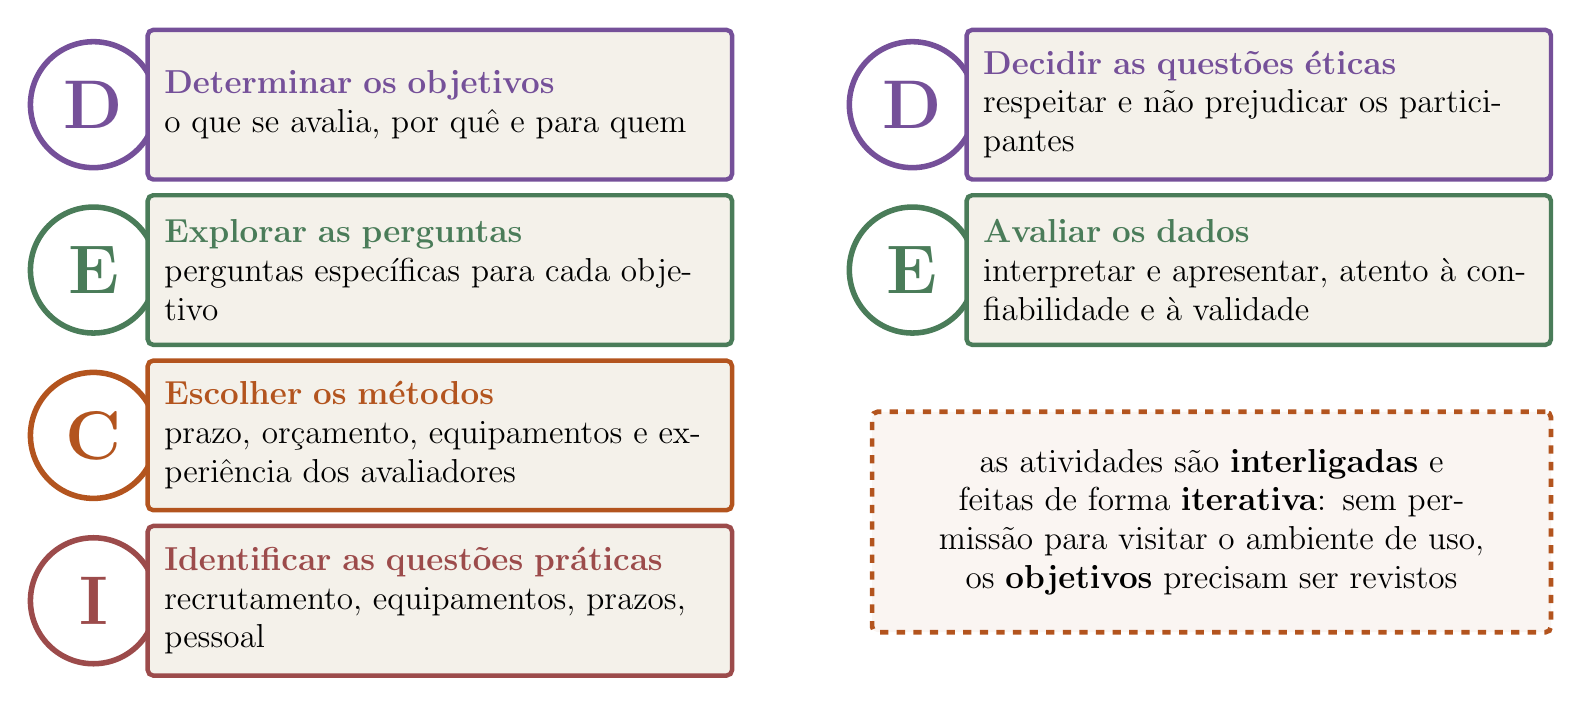
\begin{tikzpicture}[x=1cm,y=1cm]
\tikzset{l/.style={circle, minimum size=1.6cm, font=\Huge\bfseries, line width=2pt, fill=white},
        k/.style={dbox, text width=7.0cm, minimum height=1.9cm, font=\large, line width=1.6pt, align=left}}
\foreach \y/\ch/\col/\tit/\txt in {
  7.6/D/dblue/{Determinar os objetivos}/{o que se avalia, por quê e para quem},
  5.5/E/dgreen/{Explorar as perguntas}/{perguntas específicas para cada objetivo},
  3.4/C/dorange/{Escolher os métodos}/{prazo, orçamento, equipamentos e experiência dos avaliadores},
  1.3/I/dred/{Identificar as questões práticas}/{recrutamento, equipamentos, prazos, pessoal}} {
  \node[l, draw=\col, text=\col] at (1.0,\y) {\ch};
  \node[k, draw=\col] at (5.4,\y) {\textbf{\textcolor{\col}{\tit}}\\ \txt};}
\foreach \y/\ch/\col/\tit/\txt in {
  7.6/D/dblue/{Decidir as questões éticas}/{respeitar e não prejudicar os participantes},
  5.5/E/dgreen/{Avaliar os dados}/{interpretar e apresentar, atento à confiabilidade e à validade}} {
  \node[l, draw=\col, text=\col] at (11.4,\y) {\ch};
  \node[k, draw=\col] at (15.8,\y) {\textbf{\textcolor{\col}{\tit}}\\ \txt};}
\node[dbox, draw=dorange, dashed, fill=dorange!6, line width=1.7pt, text width=8.2cm, minimum height=2.8cm, font=\large] at (15.2,2.3) {as atividades são \textbf{interligadas} e feitas de forma \textbf{iterativa}: sem permissão para visitar o ambiente de uso, os \textbf{objetivos} precisam ser revistos};
\end{tikzpicture}
\end{document}
